\chapter{Logistic Regression}

Will it rain tomorrow? Will this email get opened? Will you get into the college you want? The answer is yes
or no, but the honest prediction is a probability: ``70\% chance of rain.'' \newterm{Logistic
regression}\index{logistic regression} turns numbers like humidity, hours of study, or GPA into exactly that
kind of probability.

Our running example is a real problem for field biologists. Male and female Adelie penguins look alike, and
checking a penguin's sex directly takes a blood test. Can you predict it from a scale and a ruler?

\section{Why Not a Line?}
Code the label as a number: $y = 1$ for male and $y = 0$ for female. The goal is to model
$p = P(y = 1)$, the probability that a penguin is male, from features like body mass.

You could fit a least squares line to the 0s and 1s, but look at Figure~\ref{fig:line-vs-sigmoid}. The line
predicts a probability of about $-0.2$ for the lightest Adelie and $1.4$ for the heaviest. Probabilities must stay
between 0 and 1. What we want is the S-shaped curve: flat near 0 for light penguins, flat near 1 for heavy
ones, and rising in between, where the sexes overlap.

\begin{figure}[H]
\centering
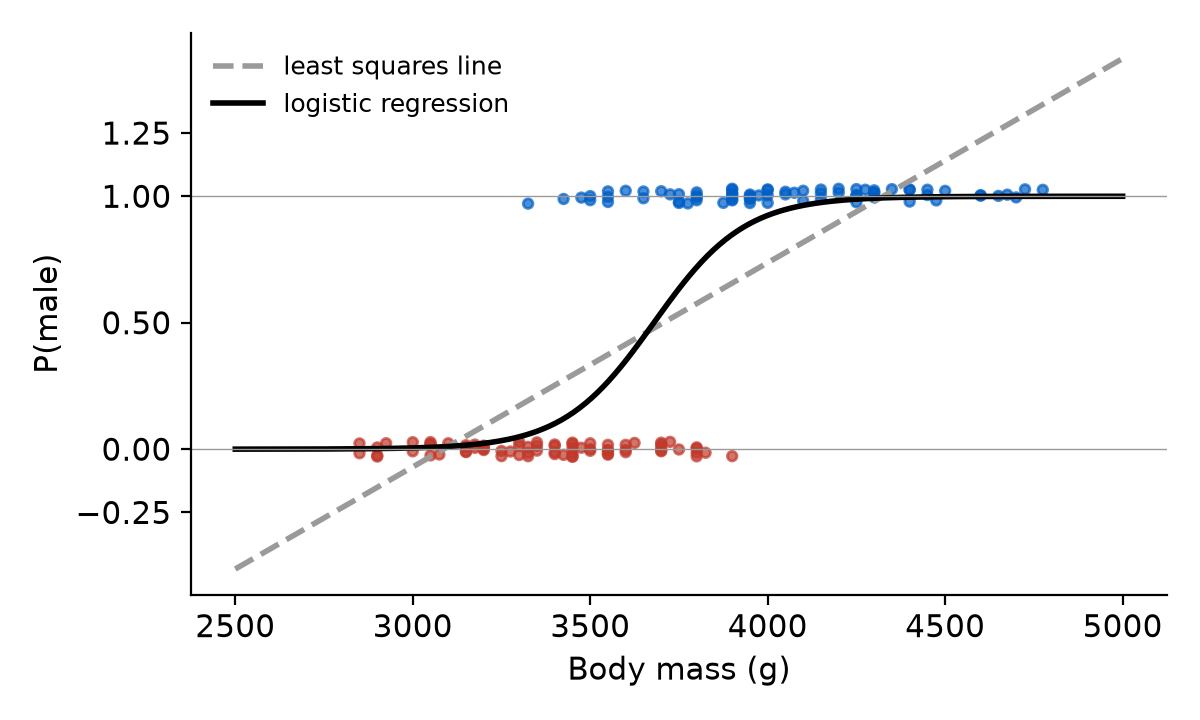
\includegraphics[width=0.72\textwidth]{line_vs_sigmoid.png}
\caption{Sex against body mass for 146 Adelie penguins (males at 1, females at 0, shaken slightly so you can
see them). The least squares line escapes the range from 0 to 1; the logistic curve does not.}
\label{fig:line-vs-sigmoid}
\end{figure}

\section{The Model}
The trick is to fit a line to something that \emph{can} take any value: the log of the odds. The
\newterm{odds} of an event are $\frac{p}{1-p}$; a probability of $0.75$ is odds of 3 (``3 to 1''). Odds run
from 0 to $\infty$, and their logarithm, the \newterm{log odds} or \newterm{logit}, runs over all real numbers.
So the model is
$$\ln\left(\frac{p}{1 - p}\right) = \beta_0 + \beta_1 x$$
Solving for $p$ gives
$$p = \sigma(\beta_0 + \beta_1 x), \qquad \text{where}\quad \sigma(z) = \frac{1}{1 + e^{-z}}$$
The function $\sigma$ is the \newterm{sigmoid}\index{sigmoid function}, or logistic function. It squeezes any
number into the range from 0 to 1, with $\sigma(0) = 0.5$.

\begin{figure}[H]
\centering
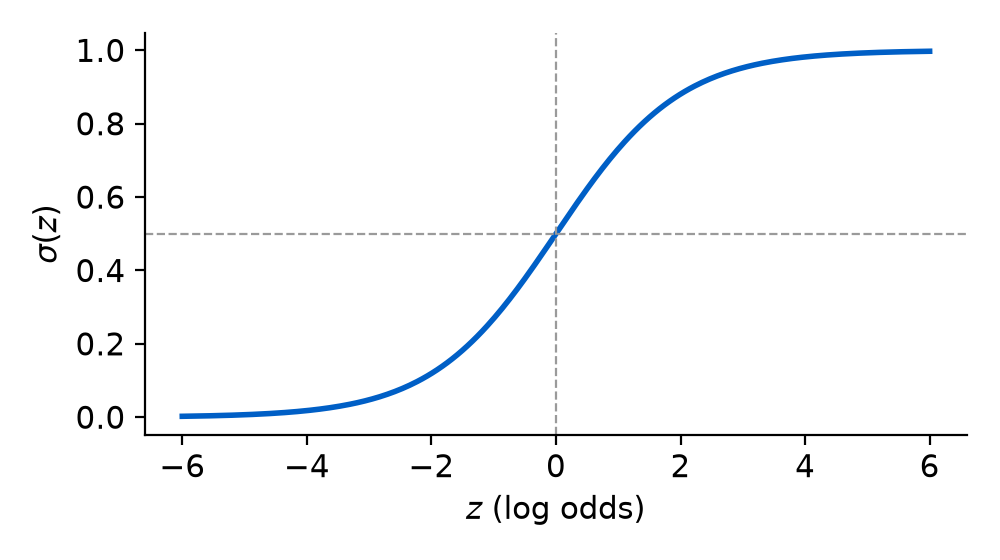
\includegraphics[width=0.55\textwidth]{sigmoid.png}
\caption{The sigmoid $\sigma(z) = 1/(1 + e^{-z})$.}
\label{fig:sigmoid}
\end{figure}

\begin{center}
\begin{tabular}{c c c}
\textbf{Probability $p$} & \textbf{Odds $p/(1-p)$} & \textbf{Log odds} \\
\hline
0.10 & 0.111 & $-2.20$ \\
0.25 & 0.333 & $-1.10$ \\
0.50 & 1 & 0 \\
0.75 & 3 & 1.10 \\
0.90 & 9 & 2.20 \\
\end{tabular}
\end{center}

\section{Interpreting the Coefficients}
Take the model $\beta_0 = -4$ and $\beta_1 = 1$. Then $p(x) = \sigma(-4 + x)$. At $x = 3$,
$p = \sigma(-1) \approx 0.269$. At $x = 4$, $p = \sigma(0) = 0.5$. At $x = 5$, $p = \sigma(1) \approx 0.731$.

Each one-unit increase in $x$ adds $\beta_1$ to the log odds, which \emph{multiplies} the odds by
$e^{\beta_1}$. Here $e^1 \approx 2.718$: the odds at $x = 3$ are $e^{-1} \approx 0.368$, at $x = 4$ they are 1,
and at $x = 5$ they are $e \approx 2.718$. The number $e^{\beta_1}$ is called the \newterm{odds
ratio}\index{odds ratio}.

\textbf{The divide-by-4 rule.} Odds ratios are hard to feel. A quick estimate: the sigmoid is steepest at its
midpoint, where its slope is $\frac{1}{4}$. So near $p = 0.5$, a one-unit increase in $x$ changes the
probability by about $\frac{\beta_1}{4}$. With $\beta_1 = 1$, that is about 25 percentage points per unit, and
indeed $p$ went from 0.5 to 0.731. The rule is only good near the middle of the curve.

\section{Several Features}\index{logistic regression!multiple}
With features $x_1, \ldots, x_p$, the log odds are a linear combination of all of them:
$$\ln\left(\frac{p}{1 - p}\right) = \beta_0 + \beta_1 x_1 + \cdots + \beta_p x_p, \qquad
p = \sigma(\beta_0 + \beta_1 x_1 + \cdots + \beta_p x_p)$$
In matrix form, with a design matrix $X$ and parameters $\boldsymbol{\theta}$ as in the last chapter, the
predicted probabilities are $\mathbf{p} = \sigma(X\boldsymbol{\theta})$, applying $\sigma$ to each entry. Each
coefficient describes one feature with the others held constant.

\textbf{Example}: A student's chance of passing an exam is modeled with hours studied $x_1$ and whether they
completed the prior course $x_2$ (1 if yes, 0 if no), with $\beta_0 = -3$, $\beta_1 = 0.5$, and $\beta_2 = 1$.
Find the probability of passing for a student who studies 4 hours and completed the prior course, and for one
who studies 2 hours and did not.

\textbf{Solution}: For the first student, the log odds are $-3 + 0.5(4) + 1 = 0$, so
$P(\text{pass}) = \sigma(0) = 0.5$. For the second, the log odds are $-3 + 0.5(2) + 0 = -2$, so
$P(\text{pass}) = \frac{1}{1 + e^{2}} \approx 0.119$. Each extra hour multiplies the odds of passing by
$e^{0.5} \approx 1.65$.

\section{Fitting: Maximum Likelihood and Log Loss}\index{maximum likelihood}\index{log loss}
Linear regression chose its parameters by least squares. For probabilities, there is a better measure of
error. If the model says a penguin is male with probability $p$, then:
\begin{itemize}
\item if the penguin is male, the model should be penalized for a \emph{small} $p$;
\item if it is female, the model should be penalized for a \emph{large} $p$.
\end{itemize}
The \newterm{log loss} (also called \newterm{cross-entropy}\index{cross-entropy}) does exactly that:
$$\text{loss} = \begin{cases} -\ln p & \text{if } y = 1 \\ -\ln(1 - p) & \text{if } y = 0 \end{cases}
\qquad\text{or, in one line,}\qquad -\big[y \ln p + (1 - y)\ln(1 - p)\big]$$

\begin{figure}[H]
\centering
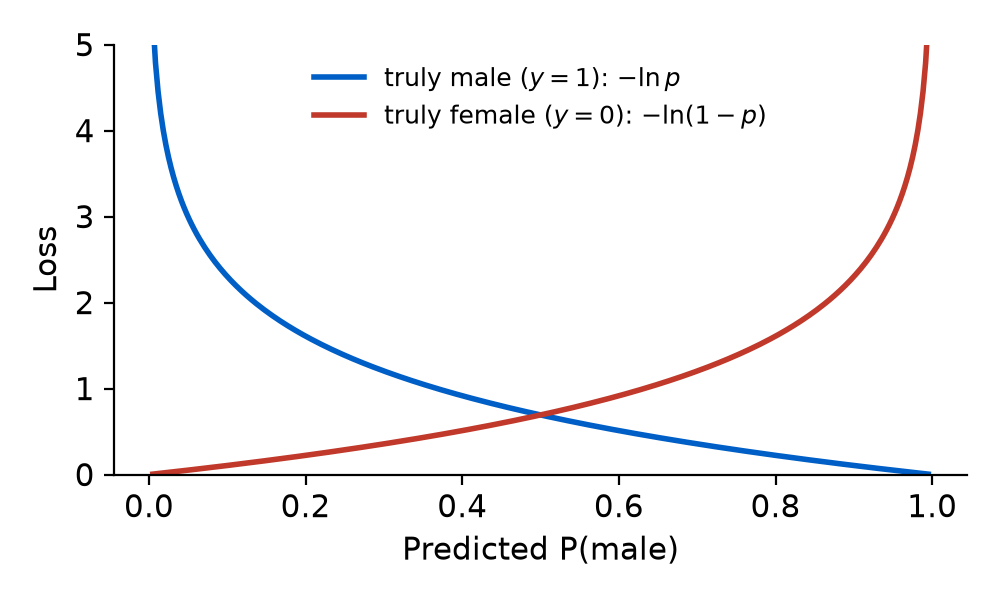
\includegraphics[width=0.55\textwidth]{log_loss.png}
\caption{Log loss for a single penguin. Being confidently wrong costs a lot.}
\label{fig:log-loss}
\end{figure}

\textbf{Example}: A model gives four penguins these probabilities of being male. Find the average log loss.

\begin{center}
\begin{tabular}{c c c c l}
\textbf{Penguin} & \textbf{True sex} & $y$ & \textbf{Predicted $p$} & \textbf{Loss} \\
\hline
A & male & 1 & 0.9 & $-\ln 0.9 = 0.105$ \\
B & male & 1 & 0.6 & $-\ln 0.6 = 0.511$ \\
C & female & 0 & 0.3 & $-\ln 0.7 = 0.357$ \\
D & female & 0 & 0.8 & $-\ln 0.2 = 1.609$ \\
\end{tabular}
\end{center}

\textbf{Solution}: The average is $(0.105 + 0.511 + 0.357 + 1.609)/4 \approx 0.646$. Penguin D, a female the
model was 80\% sure was male, contributes more than the other three together.

Minimizing the average log loss is the same as choosing the parameters that make the observed labels most
probable, which statisticians call \newterm{maximum likelihood}. Unlike least squares, there is no formula for
the answer. But the loss is a smooth bowl, so gradient descent finds the bottom, and its gradient is
remarkably simple:
$$\nabla J(\boldsymbol{\theta}) = \frac{1}{n} X^T(\mathbf{p} - \mathbf{y})$$
Compare it with linear regression's $\frac{2}{n}X^T(X\boldsymbol{\theta} - \mathbf{y})$: in both, you multiply
$X^T$ by the vector of errors, predicted minus actual.

\section{Penguins in NumPy}
Here is \filename{logistic.py}. It predicts the sex of Adelie penguins from body mass and bill depth, training
on 110 penguins and testing on 36:

\begin{minted}{python}
import numpy as np
from scipy.optimize import minimize
from penguins import load_penguins

data = load_penguins()
adelie = data["species"] == "Adelie"
y = (data["sex"][adelie] == "male").astype(float)    # 1 = male, 0 = female
features = np.column_stack([data["body_mass_g"][adelie],
                            data["bill_depth_mm"][adelie]])
n = len(y)

order = np.random.default_rng(1).permutation(n)
train, test = order[:110], order[110:]

# Standardize with the training penguins' means and standard deviations
mean, sd = features[train].mean(axis=0), features[train].std(axis=0)
X = np.column_stack([np.ones(n), (features - mean) / sd])

def sigmoid(z):
    return 1 / (1 + np.exp(-z))

def log_loss(theta, rows):
    p = sigmoid(X[rows] @ theta)
    return -np.mean(y[rows] * np.log(p) + (1 - y[rows]) * np.log(1 - p))

theta = np.zeros(3)
alpha = 0.5
for step in range(1, 1001):
    p = sigmoid(X[train] @ theta)
    gradient = X[train].T @ (p - y[train]) / len(train)
    theta = theta - alpha * gradient
    if step in (1, 10, 100, 1000):
        print(f"step {step:4d}: loss {log_loss(theta, train):.4f}")

print("theta:", np.round(theta, 2))
for name, rows in [("train", train), ("test", test)]:
    predicted = sigmoid(X[rows] @ theta) >= 0.5
    print(f"{name} accuracy: {np.mean(predicted == y[rows]):.1%}")

# A new Adelie: 3600 g, bill depth 18.0 mm
x_new = np.concatenate([[1], (np.array([3600, 18.0]) - mean) / sd])
print(f"P(male) = {sigmoid(x_new @ theta):.2f}")

# Check against SciPy's general-purpose minimizer
result = minimize(log_loss, np.zeros(3), args=(train,))
print("SciPy theta:", np.round(result.x, 2))
\end{minted}

\begin{verbatim}
step    1: loss 0.5855
step   10: loss 0.3401
step  100: loss 0.2443
step 1000: loss 0.2379
theta: [0.54 3.55 1.36]
train accuracy: 88.2%
test accuracy: 88.9%
P(male) = 0.32
SciPy theta: [0.54 3.55 1.36]
\end{verbatim}

The model sexes 32 of the 36 test penguins correctly. The baseline, always guessing the more common sex, would
get about half right. SciPy's \verb|minimize| reaches the same $\boldsymbol{\theta}$, which is a good check
that gradient descent found the bottom.

Reading the coefficients: the features are standardized, so $3.55$ is the change in log odds for a penguin one
standard deviation (474 g) heavier, with the same bill depth. Per 100 g, that is $3.55 \times 100/474 \approx
0.75$, an odds ratio of $e^{0.75} \approx 2.1$. Near a 50--50 penguin, the divide-by-4 rule says 100 g adds
about $0.75/4 \approx 19$ percentage points to the chance of being male. Mass matters more than bill depth
here, but both help.

\section{Making a Decision}\index{decision boundary}
To turn a probability into a prediction, choose a \newterm{threshold}, usually 0.5: predict male when
$p \ge 0.5$. Since $p = 0.5$ exactly when the log odds are 0, the boundary between the two predictions is
where $\theta_0 + \theta_1 x_1 + \theta_2 x_2 = 0$, a straight line. That is why logistic regression is called a
\newterm{linear classifier}.

\begin{figure}[H]
\centering
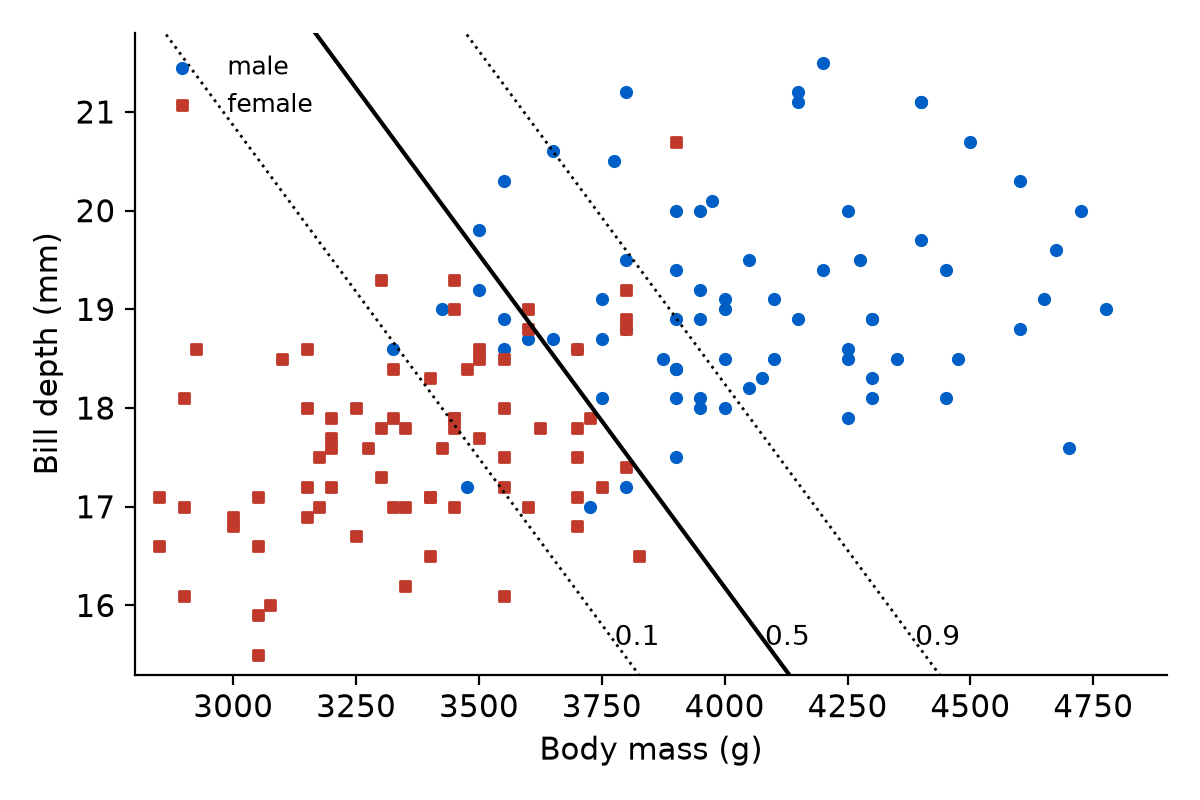
\includegraphics[width=0.72\textwidth]{boundary.png}
\caption{Lines of equal probability for a model fit to all 146 Adelies. The solid line is $P(\text{male}) =
0.5$; the dotted lines are 0.1 and 0.9.}
\label{fig:boundary}
\end{figure}

The threshold is a choice, and changing it changes which mistakes the model makes. A spam filter might demand
$p \ge 0.95$ before hiding a message, because hiding a real email is worse than letting one piece of spam
through. The next chapter is all about measuring those trade-offs.

\begin{Exercise}[label=slog1, title=Compute a probability]
Using $\beta_0 = -4$ and $\beta_1 = 1$, find $p(2)$.
\end{Exercise}
\begin{Answer}[ref=slog1]
$p(2) = \sigma(-2) = \frac{1}{1 + e^{2}} \approx \frac{1}{8.389} \approx 0.119$.
\end{Answer}

\begin{Exercise}[label=slog2, title=Find the threshold value]
With $\beta_0 = -4$ and $\beta_1 = 1$, for which $x$ is $p(x) = 0.5$?
\end{Exercise}
\begin{Answer}[ref=slog2]
$p(x) = 0.5$ when the log odds are 0, so $-4 + x = 0$. Thus $x = 4$.
\end{Answer}

\begin{Exercise}[label=slog3, title=Interpret the odds ratio]
If $\beta_1 = 0.5$, by what factor do the odds of $y = 1$ change when $x$ increases by 1?
\end{Exercise}
\begin{Answer}[ref=slog3]
The odds are multiplied by $e^{0.5} \approx 1.649$, an increase of about 65\%.
\end{Answer}

\begin{Exercise}[label=slog4, title=From odds to probability]
A model gives log odds of $0.8$ for a particular student passing. What are the odds, and what is the
probability of passing?
\end{Exercise}
\begin{Answer}[ref=slog4]
The odds are $e^{0.8} \approx 2.23$, meaning passing is about 2.23 times as likely as failing. The probability
is $\frac{2.23}{1 + 2.23} \approx 0.69$.
\end{Answer}

\begin{Exercise}[label=mlog1, title=Compute a probability]
In the exam example, find $P(\text{pass})$ for a student who studies 6 hours and did not complete the prior
course.
\end{Exercise}
\begin{Answer}[ref=mlog1]
The log odds are $-3 + 0.5(6) + 0 = 0$, so $P = 0.5$.
\end{Answer}

\begin{Exercise}[label=mlog3, title=Divide by 4]
In the exam example, the first student has $P(\text{pass}) = 0.5$. Use the divide-by-4 rule to estimate their
probability of passing if they study one more hour. Then compute it exactly.
\end{Exercise}
\begin{Answer}[ref=mlog3]
The rule says the probability rises by about $\frac{0.5}{4} = 0.125$, to about $0.625$. Exactly, the log odds
are $0.5$ and $P = \frac{1}{1 + e^{-0.5}} \approx 0.622$. The rule is very close because the student starts at
$P = 0.5$.
\end{Answer}

\begin{Exercise}[label=mlog2, title=Log loss by hand, space=3cm]
A model predicts $P(\text{male}) = 0.95$ for a penguin that is female. What is its log loss? What would the
loss be if the model had said 0.5 instead?
\end{Exercise}
\begin{Answer}[ref=mlog2]
$-\ln(1 - 0.95) = -\ln 0.05 \approx 3.00$. With 0.5, the loss is $-\ln 0.5 \approx 0.69$. Being confidently
wrong costs more than four times as much as shrugging.
\end{Answer}

\begin{Exercise}[label=mlog4, title={One feature at a time}]
Change \filename{logistic.py} to use only body mass, then only bill depth. Report the test accuracy of each.
Was it worth using both?
\end{Exercise}
\begin{Answer}[ref=mlog4]
Keep only one column of \verb|features|, for example
\begin{minted}{python}
features = data["body_mass_g"][adelie][:, None]
\end{minted}
and start from \verb|np.zeros(2)| (in both places) and drop the bill depth from \verb|x_new|. Mass alone gets
77.8\% of the test penguins right, and bill depth alone gets 75.0\%. Together they get 88.9\%, so yes: each
feature carries information the other does not.
\end{Answer}

\begin{Exercise}[label=mlog5, title={Where is the line?}]
Using the printed $\boldsymbol{\theta}$ from \filename{logistic.py}, find the body mass at which an Adelie with
an average bill depth has $P(\text{male}) = 0.5$. (The training means and standard deviations are 3720 g and
474 g for mass.)
\end{Exercise}
\begin{Answer}[ref=mlog5]
An average bill depth has a standardized value of 0, so the boundary is where $0.54 + 3.55z = 0$, at
$z \approx -0.152$. In grams, that is $3720 - 0.152 \times 474 \approx 3648$ g. Average-billed Adelies heavier
than about 3650 g are predicted male.
\end{Answer}
